\chapter{Area Plots}\label{area-plots}

In this part, we will work towards creating the area plot below. We will
take you from a basic area plot and explain all the customisations we
add to the code step-by-step.

\begin{center}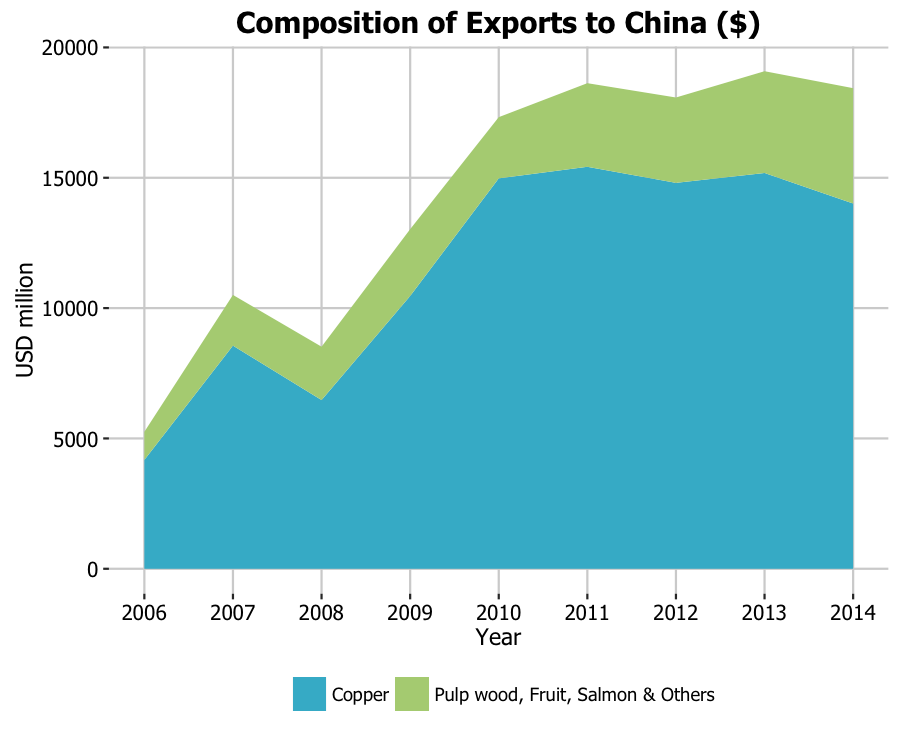
\includegraphics[width=0.55\linewidth]{0_all_posts_pdf/area_final-1} \end{center}

We will use an international trade \href{http://pachamaltese.github.io/stats/trade-chile-china/copper-data-for-tutorial.csv}{dataset} made by ourselves from different sources (Chile Customs,
Central Bank of Chile and General Directorate of International Economic Relations).

\section{Basic graph}\label{basic-graph-1}

The first thing to do is load in the data and libraries, as below:

\begin{Shaded}
\begin{Highlighting}[]
\KeywordTok{library}\NormalTok{(ggplot2)}
\KeywordTok{library}\NormalTok{(ggthemes)}
\KeywordTok{library}\NormalTok{(extrafont)}
\KeywordTok{library}\NormalTok{(plyr)}
\NormalTok{charts.data <-}\StringTok{ }\KeywordTok{read.csv}\NormalTok{(}\StringTok{"copper-data-for-tutorial.csv"}\NormalTok{)}
\end{Highlighting}
\end{Shaded}

In order to initialise a plot we tell ggplot that \texttt{charts.data}
is our data, and specify the variables on each axis. We then instruct
ggplot to render this as an area plot by adding the \texttt{geom\_area}
command.

\begin{Shaded}
\begin{Highlighting}[]
\NormalTok{charts.data <-}\StringTok{ }\KeywordTok{read.csv}\NormalTok{(}\StringTok{"copper-data-for-tutorial.csv"}\NormalTok{)}

\NormalTok{p2 <-}\StringTok{ }\KeywordTok{ggplot}\NormalTok{() +}\StringTok{ }\KeywordTok{geom_area}\NormalTok{(}\KeywordTok{aes}\NormalTok{(}\DataTypeTok{y =} \NormalTok{export, }\DataTypeTok{x =} \NormalTok{year, }\DataTypeTok{fill =} \NormalTok{product), }
\StringTok{        }\DataTypeTok{data =} \NormalTok{charts.data, }\DataTypeTok{stat=}\StringTok{"identity"}\NormalTok{)}
\NormalTok{p2}
\end{Highlighting}
\end{Shaded}

\begin{center}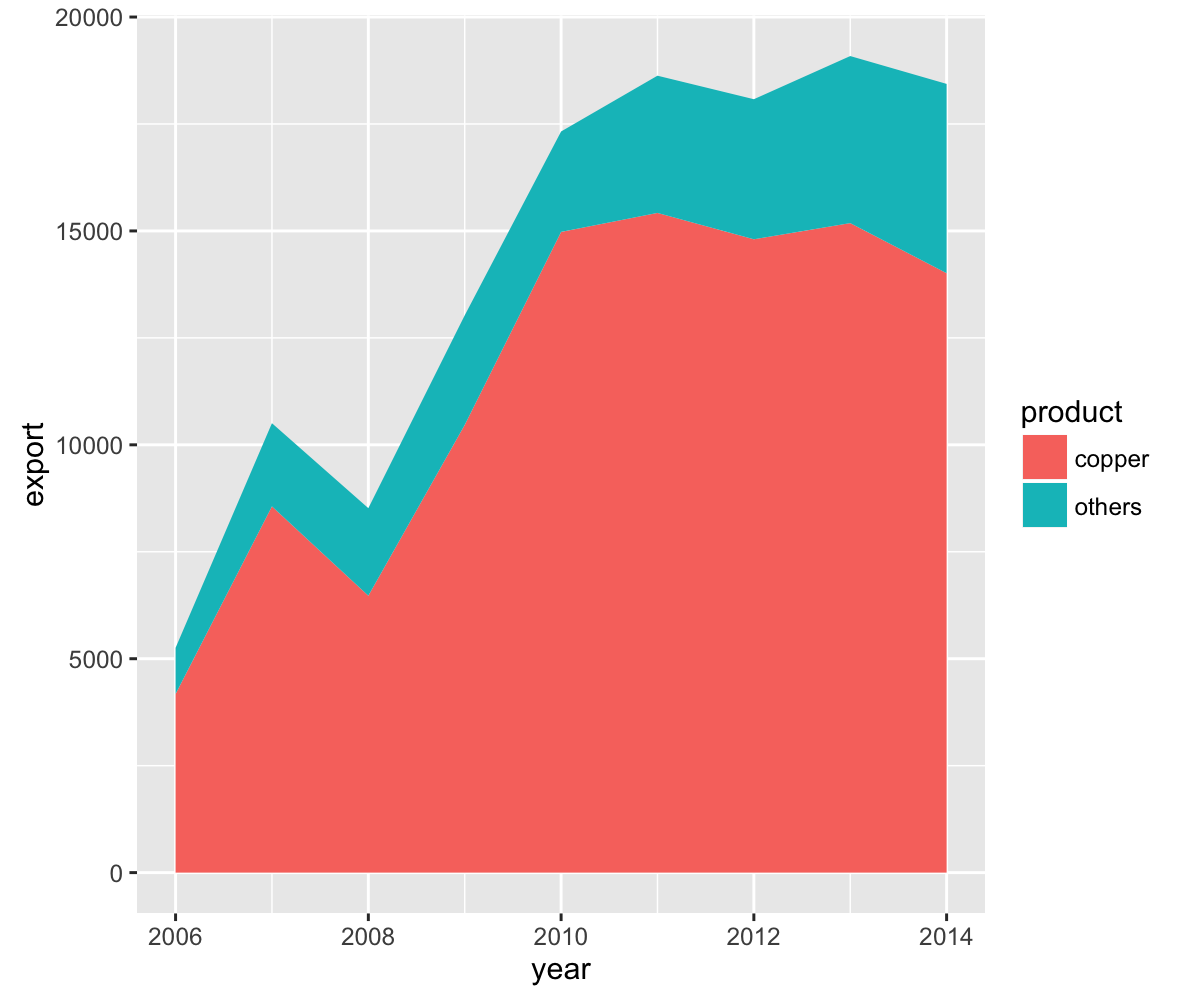
\includegraphics[width=0.55\linewidth]{0_all_posts_pdf/area_1-1} \end{center}

\section{Adjusting legend position}\label{adjusting-legend-position}

To adjust the position of the legend from the default spot of right of
the graph, we add the \texttt{theme} option and specify the
\texttt{legend.position="bottom"} argument. We can also change the title
to blank using the \texttt{legend.title\ =\ element\_blank()} argument
and change the legend shape using the
\texttt{legend.direction="horizontal"} argument.

\begin{Shaded}
\begin{Highlighting}[]
\NormalTok{charts.data <-}\StringTok{ }\KeywordTok{ddply}\NormalTok{(charts.data, .(year), transform, }
\StringTok{        }\DataTypeTok{pos =} \KeywordTok{cumsum}\NormalTok{(export) -}\StringTok{ }\NormalTok{(}\FloatTok{0.5} \NormalTok{*}\StringTok{ }\NormalTok{export))}

\NormalTok{p2 <-}\StringTok{ }\NormalTok{p2 +}\StringTok{ }\KeywordTok{theme}\NormalTok{(}\DataTypeTok{legend.position=}\StringTok{"bottom"}\NormalTok{, }\DataTypeTok{legend.direction=}\StringTok{"horizontal"}\NormalTok{, }
\StringTok{        }\DataTypeTok{legend.title =} \KeywordTok{element_blank}\NormalTok{())}
\NormalTok{p2}
\end{Highlighting}
\end{Shaded}

\begin{center}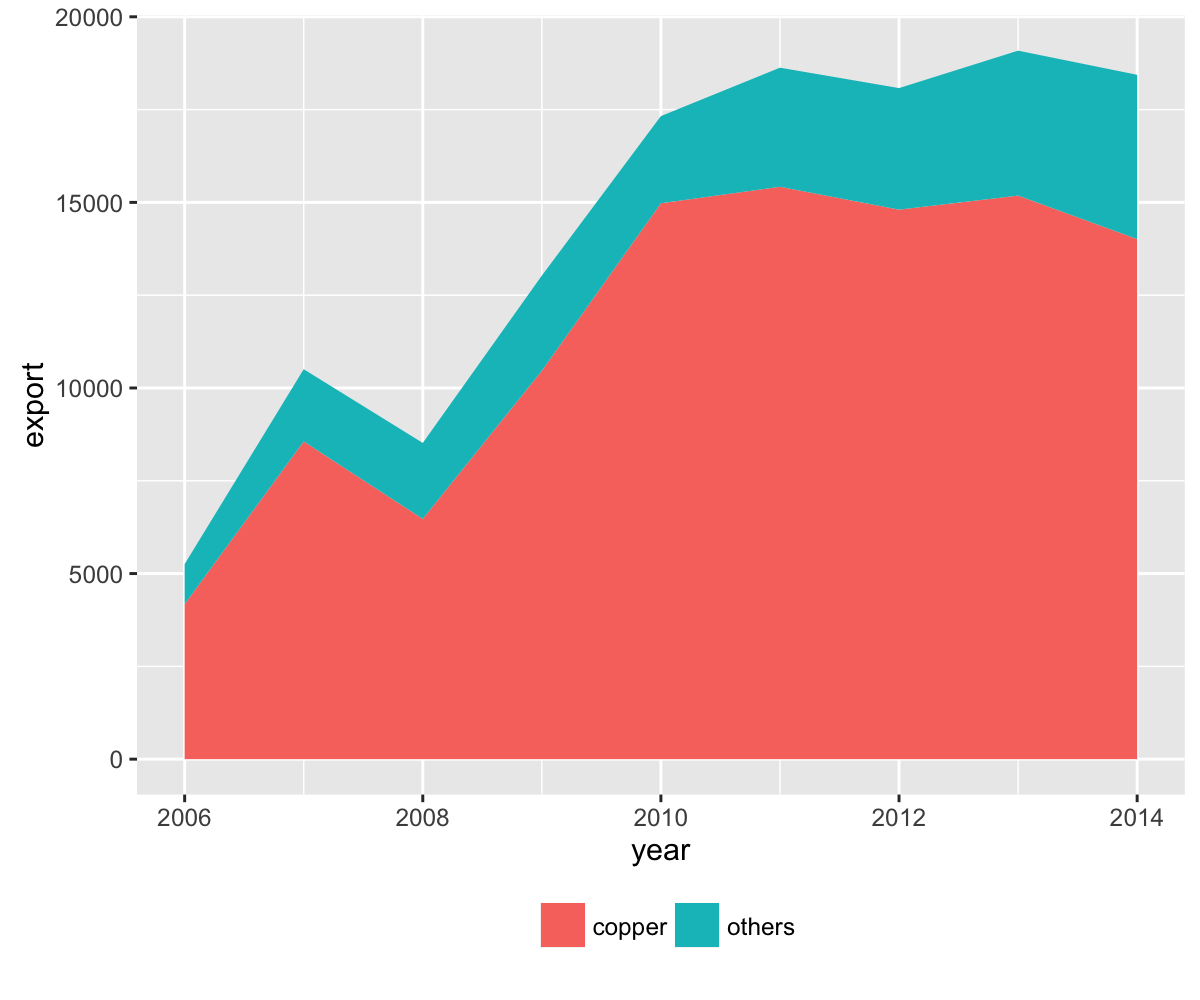
\includegraphics[width=0.55\linewidth]{0_all_posts_pdf/area_2-1} \end{center}

\section{Changing variables
display}\label{changing-variables-display-1}

To change the variables displayed name, we need to re-factor our data
labels in \texttt{charts.data} data frame.

\begin{Shaded}
\begin{Highlighting}[]
\NormalTok{charts.data <-}\StringTok{ }\KeywordTok{as.data.frame}\NormalTok{(charts.data)}
\NormalTok{charts.data$product <-}\StringTok{ }\KeywordTok{factor}\NormalTok{(charts.data$product, }
\StringTok{        }\DataTypeTok{levels =} \KeywordTok{c}\NormalTok{(}\StringTok{"copper"}\NormalTok{,}\StringTok{"others"}\NormalTok{), }
\StringTok{        }\DataTypeTok{labels =} \KeywordTok{c}\NormalTok{(}\StringTok{"Copper"}\NormalTok{,}\StringTok{"Pulp wood, Fruit, Salmon & Others"}\NormalTok{))}

\NormalTok{p2 <-}\StringTok{ }\KeywordTok{ggplot}\NormalTok{() +}\StringTok{ }
\StringTok{      }\KeywordTok{geom_area}\NormalTok{(}\KeywordTok{aes}\NormalTok{(}\DataTypeTok{y =} \NormalTok{export, }\DataTypeTok{x =} \NormalTok{year, }\DataTypeTok{fill =} \NormalTok{product), }\DataTypeTok{data =} \NormalTok{charts.data, }
\StringTok{        }\DataTypeTok{stat=}\StringTok{"identity"}\NormalTok{) +}\StringTok{ }
\StringTok{      }\KeywordTok{theme}\NormalTok{(}\DataTypeTok{legend.position=}\StringTok{"bottom"}\NormalTok{, }\DataTypeTok{legend.direction=}\StringTok{"horizontal"}\NormalTok{, }
\StringTok{        }\DataTypeTok{legend.title =} \KeywordTok{element_blank}\NormalTok{())}
\NormalTok{p2}
\end{Highlighting}
\end{Shaded}

\begin{center}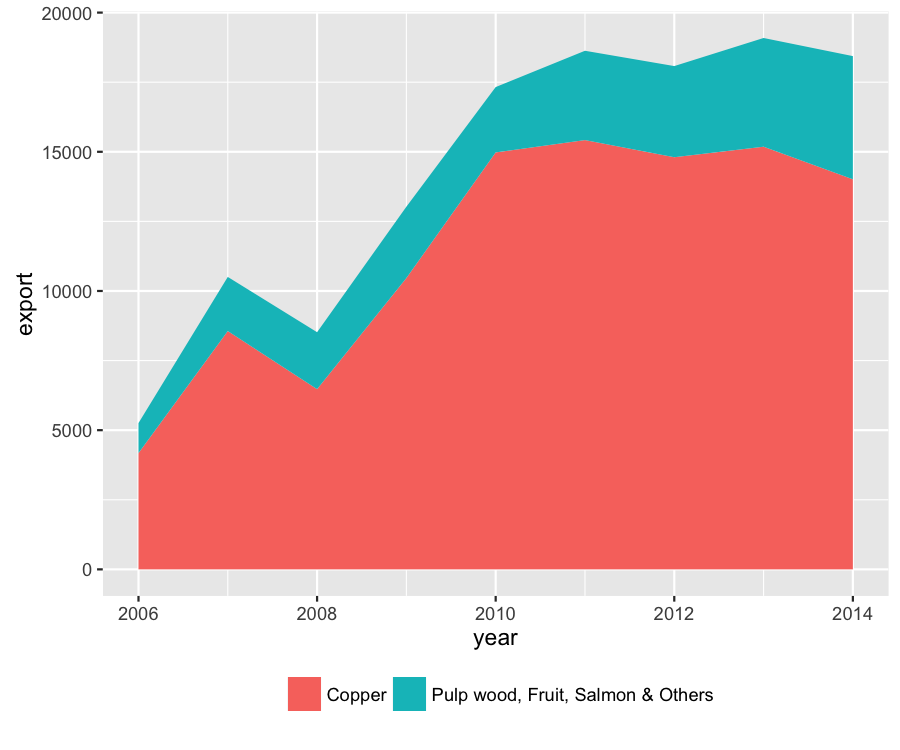
\includegraphics[width=0.55\linewidth]{0_all_posts_pdf/area_3-1} \end{center}

\section{Adjusting x-axis scale}\label{adjusting-x-axis-scale-1}

To change the axis tick marks, we use the \texttt{scale\_x\_continuous}
and/or \texttt{scale\_y\_continuous} commands.

\begin{Shaded}
\begin{Highlighting}[]
\NormalTok{p2 <-}\StringTok{ }\NormalTok{p2 +}\StringTok{ }\KeywordTok{scale_x_continuous}\NormalTok{(}\DataTypeTok{breaks=}\KeywordTok{seq}\NormalTok{(}\DecValTok{2006}\NormalTok{,}\DecValTok{2014}\NormalTok{,}\DecValTok{1}\NormalTok{))}
\NormalTok{p2}
\end{Highlighting}
\end{Shaded}

\begin{center}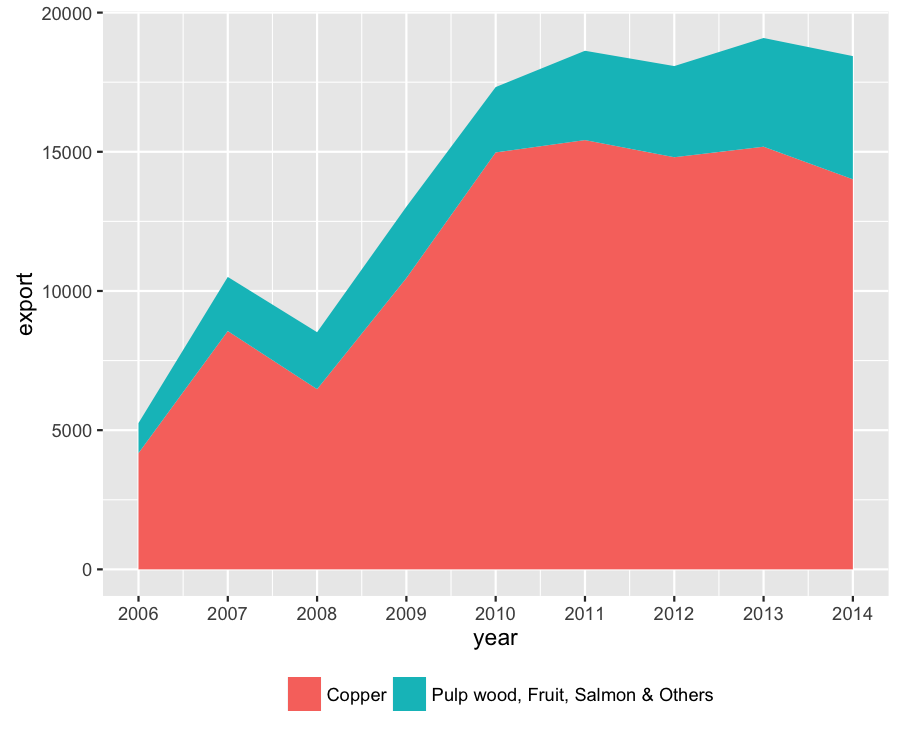
\includegraphics[width=0.55\linewidth]{0_all_posts_pdf/area_4-1} \end{center}

\section{Adjusting axis labels \& adding
title}\label{adjusting-axis-labels-adding-title-1}

To add a title, we include the option \texttt{ggtitle} and include the
name of the graph as a string argument, and to change the axis names we
use the \texttt{labs} command.

\begin{Shaded}
\begin{Highlighting}[]
\NormalTok{p2 <-}\StringTok{ }\NormalTok{p2 +}\StringTok{ }\KeywordTok{ggtitle}\NormalTok{(}\StringTok{"Composition of Exports to China ($)"}\NormalTok{) +}\StringTok{ }
\StringTok{      }\KeywordTok{labs}\NormalTok{(}\DataTypeTok{x=}\StringTok{"Year"}\NormalTok{, }\DataTypeTok{y=}\StringTok{"USD million"}\NormalTok{) }
\NormalTok{p2}
\end{Highlighting}
\end{Shaded}

\begin{center}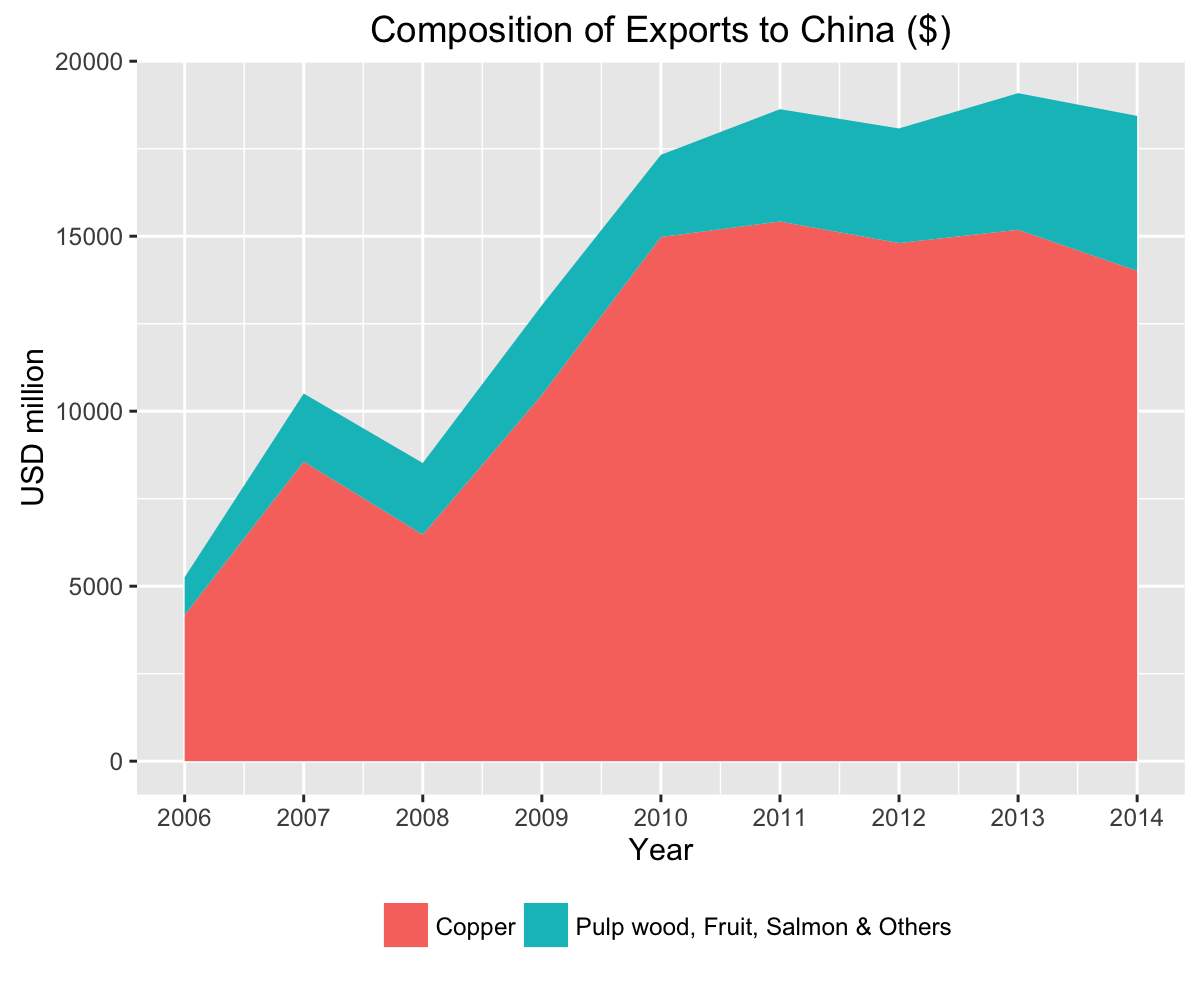
\includegraphics[width=0.55\linewidth]{0_all_posts_pdf/area_5-1} \end{center}

\section{Adjusting color palette}\label{adjusting-color-palette-1}

To change the colours, we use the \texttt{scale\_colour\_manual}
command. Note that you can reference the specific colours you'd like to
use with specific HEX codes. You can also reference colours by name,
with the full list of colours recognised by R
\href{http://www.stat.columbia.edu/~tzheng/files/Rcolor.pdf}{here}.

\begin{Shaded}
\begin{Highlighting}[]
\NormalTok{fill <-}\StringTok{ }\KeywordTok{c}\NormalTok{(}\StringTok{"#5F9EA0"}\NormalTok{, }\StringTok{"#E1B378"}\NormalTok{)}
\NormalTok{p2 <-}\StringTok{ }\NormalTok{p2 +}\StringTok{ }\KeywordTok{scale_fill_manual}\NormalTok{(}\DataTypeTok{values=}\NormalTok{fill)}
\NormalTok{p2}
\end{Highlighting}
\end{Shaded}

\begin{center}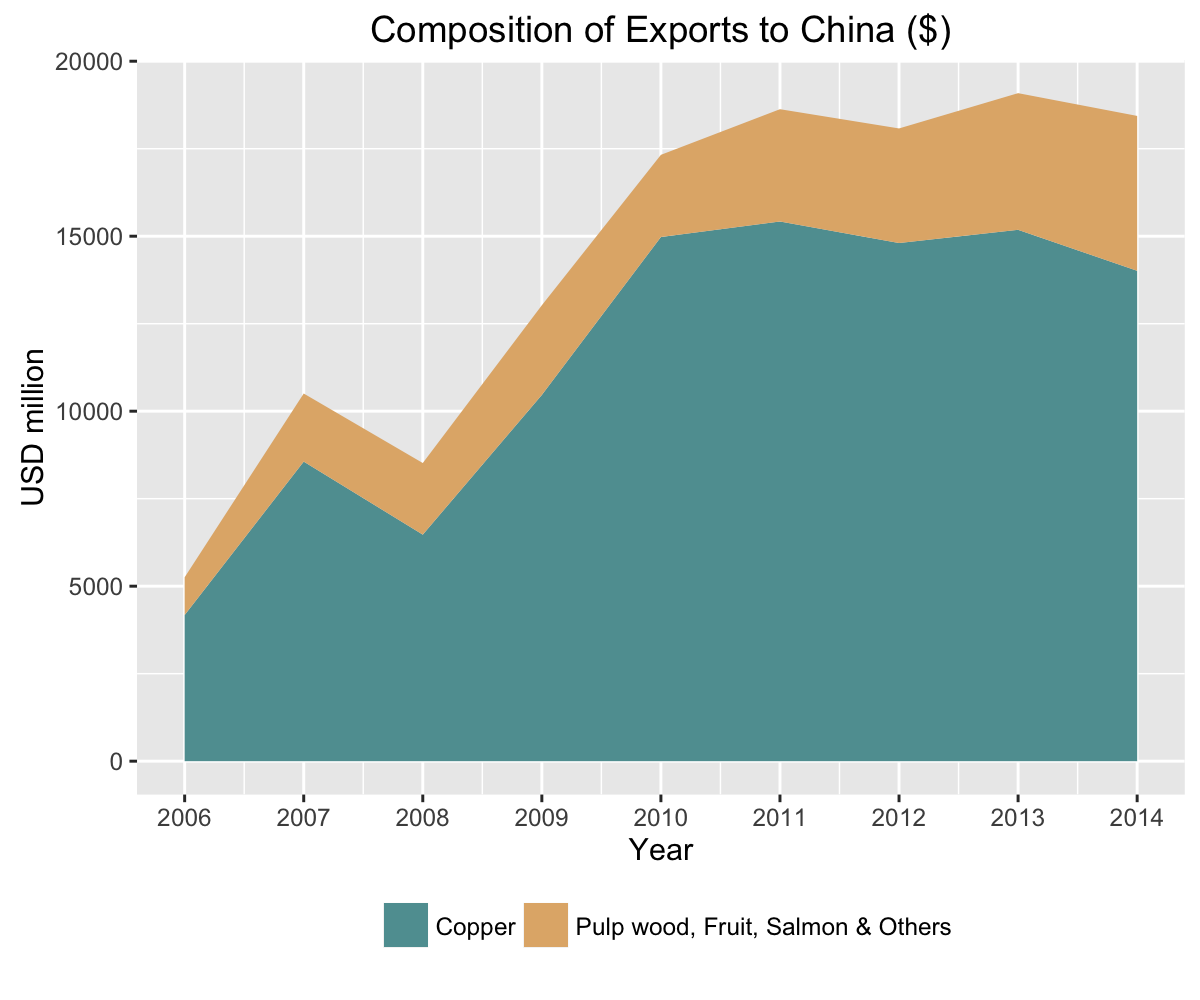
\includegraphics[width=0.55\linewidth]{0_all_posts_pdf/area_6-1} \end{center}

\section{Using the white theme}\label{using-the-white-theme-1}

As explained in the previous post, we can also change the overall look
of the site using themes. We'll start using a simple theme customisation
by adding \texttt{theme\_bw()} after \texttt{ggplot()}. As you can see,
we can further tweak the graph using the \texttt{theme} option, which
we've used so far to change the legend.

\begin{Shaded}
\begin{Highlighting}[]
\NormalTok{p2 <-}\StringTok{ }\KeywordTok{ggplot}\NormalTok{() +}
\StringTok{      }\KeywordTok{geom_area}\NormalTok{(}\KeywordTok{aes}\NormalTok{(}\DataTypeTok{y =} \NormalTok{export, }\DataTypeTok{x =} \NormalTok{year, }\DataTypeTok{fill =} \NormalTok{product), }\DataTypeTok{data =} \NormalTok{charts.data, }
\StringTok{        }\DataTypeTok{stat=}\StringTok{"identity"}\NormalTok{) +}\StringTok{ }
\StringTok{      }\KeywordTok{scale_x_continuous}\NormalTok{(}\DataTypeTok{breaks=}\KeywordTok{seq}\NormalTok{(}\DecValTok{2006}\NormalTok{,}\DecValTok{2014}\NormalTok{,}\DecValTok{1}\NormalTok{)) +}\StringTok{ }
\StringTok{      }\KeywordTok{labs}\NormalTok{(}\DataTypeTok{x=}\StringTok{"Year"}\NormalTok{, }\DataTypeTok{y=}\StringTok{"USD million"}\NormalTok{) +}\StringTok{ }
\StringTok{      }\KeywordTok{ggtitle}\NormalTok{(}\StringTok{"Composition of Exports to China ($)"}\NormalTok{) +}\StringTok{ }
\StringTok{      }\KeywordTok{scale_fill_manual}\NormalTok{(}\DataTypeTok{values=}\NormalTok{fill) +}
\StringTok{      }\KeywordTok{theme_bw}\NormalTok{() +}
\StringTok{      }\KeywordTok{theme}\NormalTok{(}\DataTypeTok{legend.position=}\StringTok{"bottom"}\NormalTok{, }
\StringTok{        }\DataTypeTok{legend.direction=}\StringTok{"horizontal"}\NormalTok{, }
\StringTok{        }\DataTypeTok{legend.title =} \KeywordTok{element_blank}\NormalTok{())   }
\NormalTok{p2}
\end{Highlighting}
\end{Shaded}

\begin{center}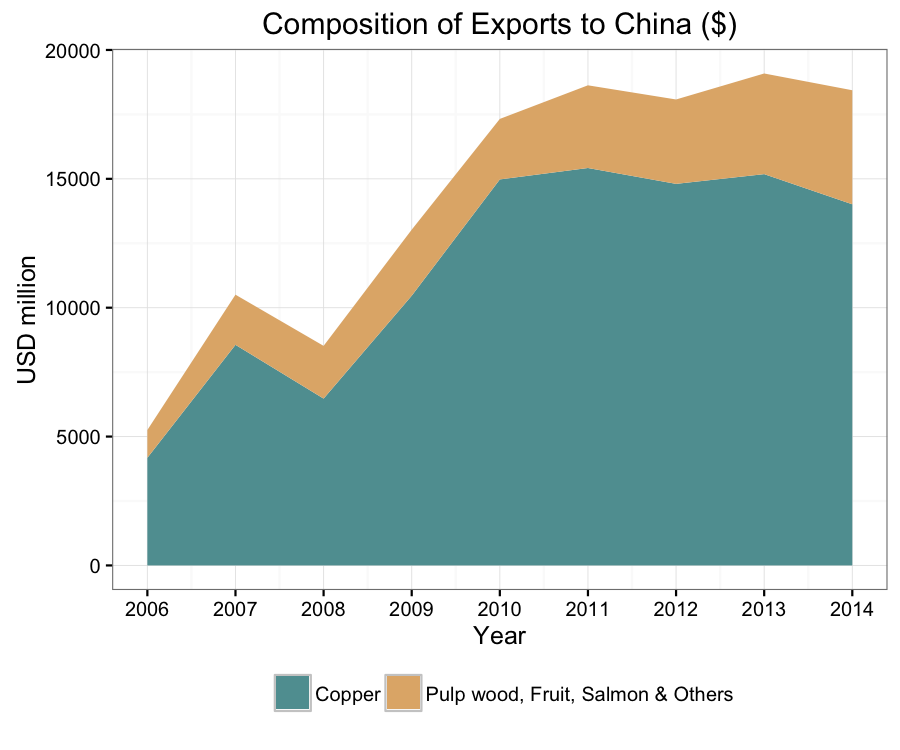
\includegraphics[width=0.55\linewidth]{0_all_posts_pdf/area_7-1} \end{center}

\section{Creating an XKCD style
chart}\label{creating-an-xkcd-style-chart-1}

Of course, you may want to create your own themes as well.
\texttt{ggplot2} allows for a very high degree of customisation,
including allowing you to use imported fonts. Below is an example of a
theme Mauricio was able to create which mimics the visual style of
\href{http://xkcd.com/}{XKCD}. In order to create this chart, you first
need to import the XKCD font, install it on your machine and load it
into R using the \texttt{extrafont} package. These instructions are
taken from
\href{https://www.google.com.au/url?sa=t\&rct=j\&q=\&esrc=s\&source=web\&cd=1\&ved=0ahUKEwiWzafchdPJAhVBpJQKHe_LDT8QFggbMAA\&url=https\%3A\%2F\%2Fcran.r-project.org\%2Fweb\%2Fpackages\%2Fxkcd\%2Fvignettes\%2Fxkcd-intro.pdf\&usg=AFQjCNE-KciGY14e-Q1buYIVmTFC0ht__Q\&sig2=DZUwkvIHwfNWtTtkcz94jg}{here}:

\begin{Shaded}
\begin{Highlighting}[]
\KeywordTok{library}\NormalTok{(extrafont)}

\KeywordTok{download.file}\NormalTok{(}\StringTok{"http://simonsoftware.se/other/xkcd.ttf"}\NormalTok{, }
\StringTok{      }\DataTypeTok{dest=}\StringTok{"xkcd.ttf"}\NormalTok{, }\DataTypeTok{mode=}\StringTok{"wb"}\NormalTok{)}
\KeywordTok{system}\NormalTok{(}\StringTok{"mkdir ~/.fonts"}\NormalTok{)}
\KeywordTok{system}\NormalTok{(}\StringTok{"cp xkcd.ttf  ~/.fonts"}\NormalTok{)}
\KeywordTok{font_import}\NormalTok{(}\DataTypeTok{paths =} \StringTok{"~/.fonts"}\NormalTok{, }\DataTypeTok{pattern=}\StringTok{"[X/x]kcd"}\NormalTok{)}
\KeywordTok{fonts}\NormalTok{()}
\KeywordTok{loadfonts}\NormalTok{()}
\end{Highlighting}
\end{Shaded}

You can then create your graph:

\begin{Shaded}
\begin{Highlighting}[]
\NormalTok{fill <-}\StringTok{ }\KeywordTok{c}\NormalTok{(}\StringTok{"#56B4E9"}\NormalTok{, }\StringTok{"#ffcc00"}\NormalTok{)}

\NormalTok{p2 <-}\StringTok{ }\KeywordTok{ggplot}\NormalTok{() +}\StringTok{ }
\StringTok{      }\KeywordTok{geom_area}\NormalTok{(}\KeywordTok{aes}\NormalTok{(}\DataTypeTok{y =} \NormalTok{export, }\DataTypeTok{x =} \NormalTok{year, }\DataTypeTok{fill =} \NormalTok{product), }\DataTypeTok{data =} \NormalTok{charts.data, }
\StringTok{        }\DataTypeTok{stat=}\StringTok{"identity"}\NormalTok{) +}\StringTok{ }
\StringTok{      }\KeywordTok{scale_x_continuous}\NormalTok{(}\DataTypeTok{breaks=}\KeywordTok{seq}\NormalTok{(}\DecValTok{2006}\NormalTok{,}\DecValTok{2014}\NormalTok{,}\DecValTok{1}\NormalTok{)) +}\StringTok{ }
\StringTok{      }\KeywordTok{labs}\NormalTok{(}\DataTypeTok{x=}\StringTok{"Year"}\NormalTok{, }\DataTypeTok{y=}\StringTok{"USD million"}\NormalTok{) +}\StringTok{ }
\StringTok{      }\KeywordTok{ggtitle}\NormalTok{(}\StringTok{"Composition of Exports to China ($)"}\NormalTok{) +}\StringTok{ }
\StringTok{      }\KeywordTok{scale_fill_manual}\NormalTok{(}\DataTypeTok{values=}\NormalTok{fill) +}\StringTok{ }
\StringTok{      }\KeywordTok{theme}\NormalTok{(}\DataTypeTok{axis.text.x=}\KeywordTok{element_text}\NormalTok{(}\DataTypeTok{colour=}\StringTok{"black"}\NormalTok{, }\DataTypeTok{size =} \DecValTok{10}\NormalTok{), }
\StringTok{        }\DataTypeTok{axis.text.y=}\KeywordTok{element_text}\NormalTok{(}\DataTypeTok{colour=}\StringTok{"black"}\NormalTok{, }\DataTypeTok{size =} \DecValTok{10}\NormalTok{),}
\StringTok{        }\DataTypeTok{axis.line.x =} \KeywordTok{element_line}\NormalTok{(}\DataTypeTok{size=}\NormalTok{.}\DecValTok{5}\NormalTok{, }\DataTypeTok{colour =} \StringTok{"black"}\NormalTok{),}
\StringTok{        }\DataTypeTok{axis.line.y =} \KeywordTok{element_line}\NormalTok{(}\DataTypeTok{size=}\NormalTok{.}\DecValTok{5}\NormalTok{, }\DataTypeTok{colour =} \StringTok{"black"}\NormalTok{),}
\StringTok{        }\DataTypeTok{legend.key=}\KeywordTok{element_rect}\NormalTok{(}\DataTypeTok{fill=}\StringTok{"white"}\NormalTok{, }\DataTypeTok{colour=}\StringTok{"white"}\NormalTok{),}
\StringTok{        }\DataTypeTok{legend.position=}\StringTok{"bottom"}\NormalTok{, }\DataTypeTok{legend.direction=}\StringTok{"horizontal"}\NormalTok{, }
\StringTok{        }\DataTypeTok{legend.title =} \KeywordTok{element_blank}\NormalTok{(),}
\StringTok{        }\DataTypeTok{panel.grid.major =} \KeywordTok{element_blank}\NormalTok{(),}
\StringTok{        }\DataTypeTok{panel.grid.minor =} \KeywordTok{element_blank}\NormalTok{(), }\DataTypeTok{panel.border =} \KeywordTok{element_blank}\NormalTok{(), }
\StringTok{        }\DataTypeTok{panel.background =} \KeywordTok{element_blank}\NormalTok{(),}
\StringTok{        }\DataTypeTok{plot.title=}\KeywordTok{element_text}\NormalTok{(}\DataTypeTok{family=}\StringTok{"xkcd-Regular"}\NormalTok{), }
\StringTok{        }\DataTypeTok{text=}\KeywordTok{element_text}\NormalTok{(}\DataTypeTok{family=}\StringTok{"xkcd-Regular"}\NormalTok{)) }
\NormalTok{p2}
\end{Highlighting}
\end{Shaded}

\begin{center}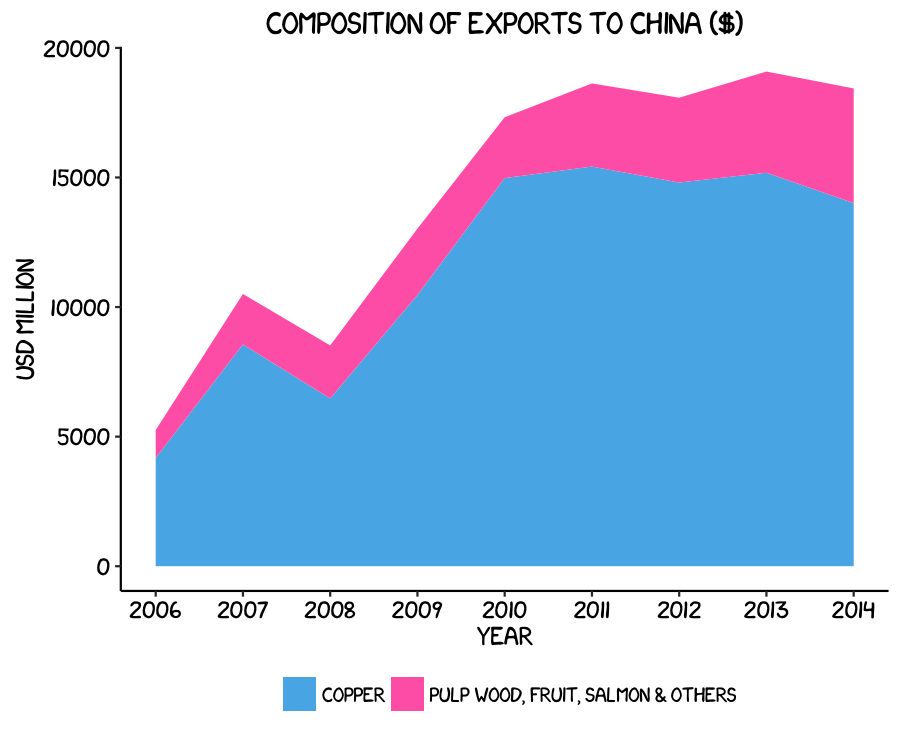
\includegraphics[width=0.55\linewidth]{0_all_posts_pdf/area_8-1} \end{center}

\section{\texorpdfstring{Using `The Economist'
theme}{Using The Economist theme}}\label{using-the-economist-theme-1}

There are a wider range of pre-built themes available as part of the
\texttt{ggthemes} package (more information on these
\href{https://cran.r-project.org/web/packages/ggthemes/vignettes/ggthemes.html}{here}).
Below we've applied \texttt{theme\_economist()}, which approximates
graphs in the Economist magazine. It is also important that the font
change argument inside \texttt{theme} is optional and it's only to
obtain a more similar result compared to the original. For an exact
result you need `Officina Sans' which is a commercial font and is
available \href{http://www.myfonts.com/fonts/itc/officina-sans/}{here}.

\begin{Shaded}
\begin{Highlighting}[]
\NormalTok{p2 <-}\StringTok{ }\KeywordTok{ggplot}\NormalTok{() +}
\StringTok{      }\KeywordTok{geom_area}\NormalTok{(}\KeywordTok{aes}\NormalTok{(}\DataTypeTok{y =} \NormalTok{export, }\DataTypeTok{x =} \NormalTok{year, }\DataTypeTok{fill =} \NormalTok{product), }\DataTypeTok{data =} \NormalTok{charts.data, }
\StringTok{        }\DataTypeTok{stat=}\StringTok{"identity"}\NormalTok{) +}\StringTok{ }
\StringTok{      }\KeywordTok{scale_x_continuous}\NormalTok{(}\DataTypeTok{breaks=}\KeywordTok{seq}\NormalTok{(}\DecValTok{2006}\NormalTok{,}\DecValTok{2014}\NormalTok{,}\DecValTok{1}\NormalTok{)) +}\StringTok{ }
\StringTok{      }\KeywordTok{labs}\NormalTok{(}\DataTypeTok{x=}\StringTok{"Year"}\NormalTok{, }\DataTypeTok{y=}\StringTok{"USD million"}\NormalTok{) +}\StringTok{ }
\StringTok{      }\KeywordTok{ggtitle}\NormalTok{(}\StringTok{"Composition of Exports to China ($)"}\NormalTok{) +}
\StringTok{      }\KeywordTok{theme_economist}\NormalTok{() +}\StringTok{ }\KeywordTok{scale_fill_economist}\NormalTok{() +}
\StringTok{      }\KeywordTok{theme}\NormalTok{(}\DataTypeTok{axis.line.x =} \KeywordTok{element_line}\NormalTok{(}\DataTypeTok{size=}\NormalTok{.}\DecValTok{5}\NormalTok{, }\DataTypeTok{colour =} \StringTok{"black"}\NormalTok{), }
\StringTok{        }\DataTypeTok{axis.line.y =} \KeywordTok{element_line}\NormalTok{(}\DataTypeTok{size=}\NormalTok{.}\DecValTok{5}\NormalTok{, }\DataTypeTok{colour =} \StringTok{"black"}\NormalTok{),}
\StringTok{        }\DataTypeTok{legend.position=}\StringTok{"bottom"}\NormalTok{, }
\StringTok{        }\DataTypeTok{legend.direction=}\StringTok{"horizontal"}\NormalTok{, }
\StringTok{        }\DataTypeTok{legend.title =} \KeywordTok{element_blank}\NormalTok{(),}
\StringTok{        }\DataTypeTok{plot.title=}\KeywordTok{element_text}\NormalTok{(}\DataTypeTok{family=}\StringTok{"OfficinaSanITC-Book"}\NormalTok{),}
\StringTok{        }\DataTypeTok{text=}\KeywordTok{element_text}\NormalTok{(}\DataTypeTok{family=}\StringTok{"OfficinaSanITC-Book"}\NormalTok{))   }
\NormalTok{p2}
\end{Highlighting}
\end{Shaded}

\begin{center}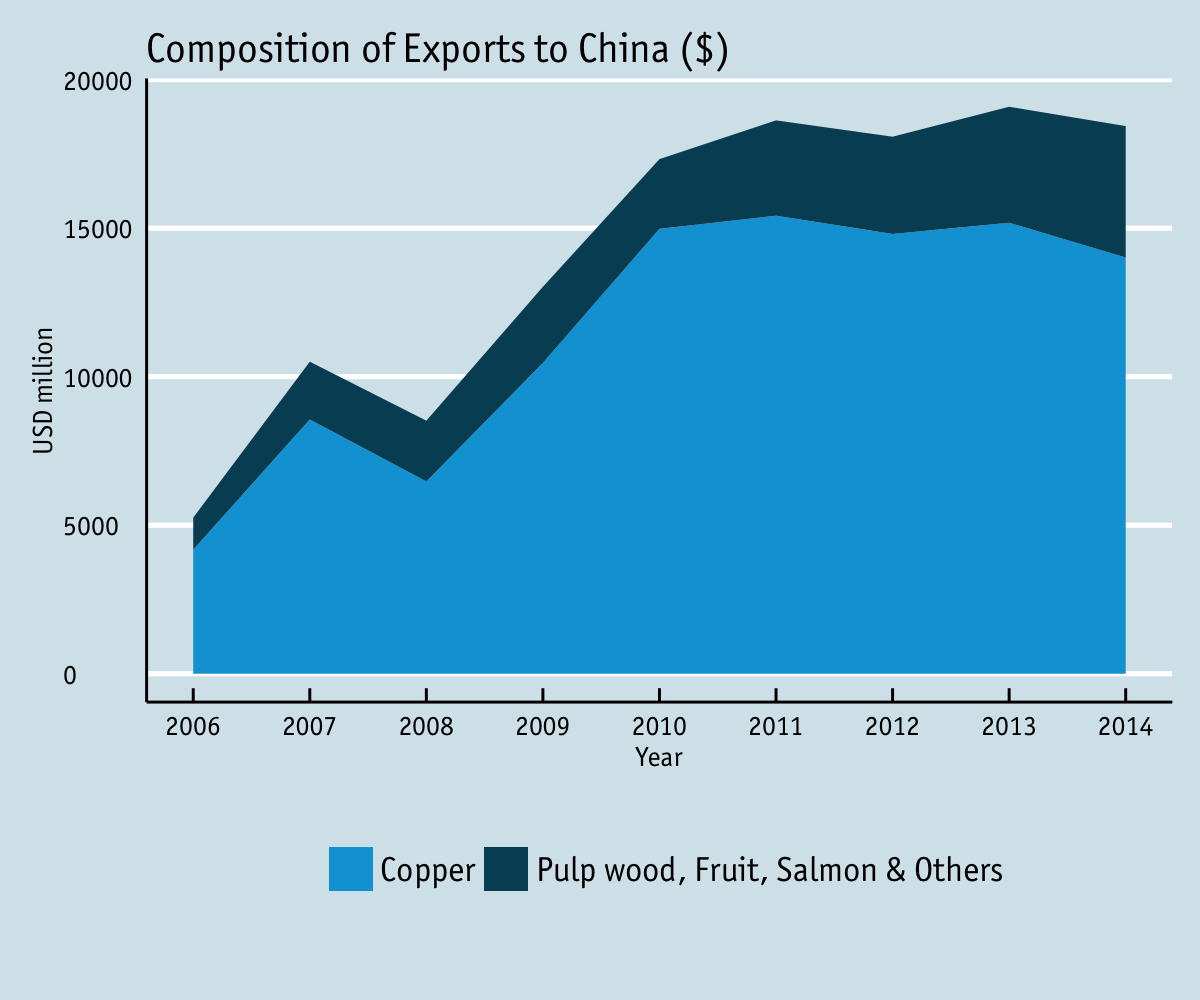
\includegraphics[width=0.55\linewidth]{0_all_posts_pdf/area_9-1} \end{center}

\section{Creating your own theme}\label{creating-your-own-theme-1}

As before, you can modify your plots a lot as \texttt{ggplot2} allows
many customisations. Here we present our original result shown at the
top of page.

\begin{Shaded}
\begin{Highlighting}[]
\NormalTok{fill <-}\StringTok{ }\KeywordTok{c}\NormalTok{(}\StringTok{"#40b8d0"}\NormalTok{, }\StringTok{"#b2d183"}\NormalTok{)}

\NormalTok{p2 <-}\StringTok{ }\KeywordTok{ggplot}\NormalTok{() +}\StringTok{ }
\StringTok{      }\KeywordTok{geom_area}\NormalTok{(}\KeywordTok{aes}\NormalTok{(}\DataTypeTok{y =} \NormalTok{export, }\DataTypeTok{x =} \NormalTok{year, }\DataTypeTok{fill =} \NormalTok{product), }\DataTypeTok{data =} \NormalTok{charts.data, }
\StringTok{        }\DataTypeTok{stat=}\StringTok{"identity"}\NormalTok{) +}\StringTok{ }
\StringTok{      }\KeywordTok{scale_x_continuous}\NormalTok{(}\DataTypeTok{breaks=}\KeywordTok{seq}\NormalTok{(}\DecValTok{2006}\NormalTok{,}\DecValTok{2014}\NormalTok{,}\DecValTok{1}\NormalTok{)) +}\StringTok{ }
\StringTok{      }\KeywordTok{labs}\NormalTok{(}\DataTypeTok{x=}\StringTok{"Year"}\NormalTok{, }\DataTypeTok{y=}\StringTok{"USD million"}\NormalTok{) +}\StringTok{ }
\StringTok{      }\KeywordTok{ggtitle}\NormalTok{(}\StringTok{"Composition of Exports to China ($)"}\NormalTok{) +}\StringTok{ }
\StringTok{      }\KeywordTok{scale_fill_manual}\NormalTok{(}\DataTypeTok{values=}\NormalTok{fill) +}\StringTok{ }
\StringTok{      }\KeywordTok{theme}\NormalTok{(}\DataTypeTok{axis.line.x =} \KeywordTok{element_line}\NormalTok{(}\DataTypeTok{size=}\NormalTok{.}\DecValTok{5}\NormalTok{, }\DataTypeTok{colour =} \StringTok{"black"}\NormalTok{), }
\StringTok{        }\DataTypeTok{axis.line.y =} \KeywordTok{element_line}\NormalTok{(}\DataTypeTok{size=}\NormalTok{.}\DecValTok{5}\NormalTok{, }\DataTypeTok{colour =} \StringTok{"black"}\NormalTok{), }
\StringTok{        }\DataTypeTok{axis.text.x=}\KeywordTok{element_text}\NormalTok{(}\DataTypeTok{colour=}\StringTok{"black"}\NormalTok{, }\DataTypeTok{size =} \DecValTok{10}\NormalTok{), }
\StringTok{        }\DataTypeTok{axis.text.y=}\KeywordTok{element_text}\NormalTok{(}\DataTypeTok{colour=}\StringTok{"black"}\NormalTok{, }\DataTypeTok{size =} \DecValTok{10}\NormalTok{),}
\StringTok{        }\DataTypeTok{legend.key=}\KeywordTok{element_rect}\NormalTok{(}\DataTypeTok{fill=}\StringTok{"white"}\NormalTok{, }\DataTypeTok{colour=}\StringTok{"white"}\NormalTok{),}
\StringTok{        }\DataTypeTok{legend.position=}\StringTok{"bottom"}\NormalTok{, }\DataTypeTok{legend.direction=}\StringTok{"horizontal"}\NormalTok{, }
\StringTok{        }\DataTypeTok{legend.title =} \KeywordTok{element_blank}\NormalTok{(),}
\StringTok{        }\DataTypeTok{panel.grid.major =} \KeywordTok{element_line}\NormalTok{(}\DataTypeTok{colour =} \StringTok{"#d3d3d3"}\NormalTok{), }
\StringTok{        }\DataTypeTok{panel.grid.minor =} \KeywordTok{element_blank}\NormalTok{(), }
\StringTok{        }\DataTypeTok{panel.border =} \KeywordTok{element_blank}\NormalTok{(), }
\StringTok{        }\DataTypeTok{panel.background =} \KeywordTok{element_blank}\NormalTok{(),}
\StringTok{        }\DataTypeTok{plot.title =} \KeywordTok{element_text}\NormalTok{(}\DataTypeTok{size =} \DecValTok{14}\NormalTok{, }\DataTypeTok{family =} \StringTok{"Tahoma"}\NormalTok{, }\DataTypeTok{face =} \StringTok{"bold"}\NormalTok{), }
\StringTok{        }\DataTypeTok{text=}\KeywordTok{element_text}\NormalTok{(}\DataTypeTok{family=}\StringTok{"Tahoma"}\NormalTok{))}
\NormalTok{p2}
\end{Highlighting}
\end{Shaded}

\begin{center}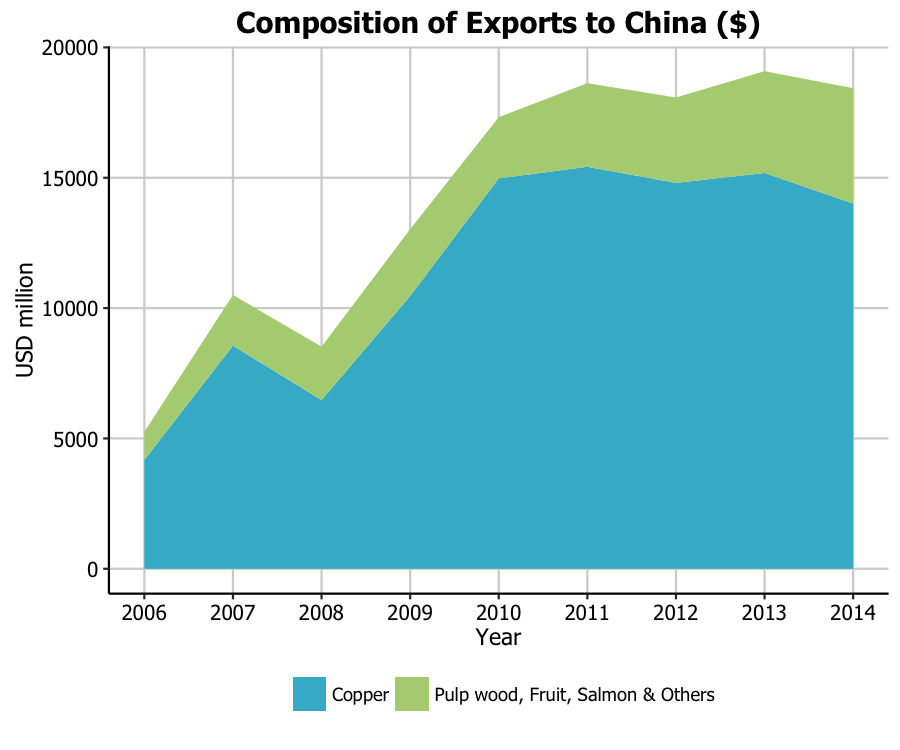
\includegraphics[width=0.55\linewidth]{0_all_posts_pdf/area_11-1} \end{center}